\documentclass[12pt]{article}
\usepackage{amsmath}
\usepackage[left=2cm,top=1cm,right=3cm,bottom=1cm]{geometry}
\usepackage{graphicx}
\usepackage{listings}


\begin{document}

\begin{center}\LARGE\bf
    Sorting
\end{center}

\section{Insertion Sort}
Insertion Sort solves the sorting problem:
\newline\textbf{Input}: A sequence of n numbers $\left\langle a_1, a_2, ..., a_n\right\rangle$
\newline\textbf{Output}: A permutation of the input sequence $\left\langle a_1', a_2', ..., a_n' \right\rangle$ where $a_1' \leq  a_2' \leq ... \leq a_n'$.

The numbers to be sorted are known as \textit{keys}. These keys are often associated with other data, which we call \textit{satellite data}. A
key and satellite data form a \textit{record}. When sorting with respect to some key, the satellite data is also sorted so that it stays with the associated
key.

In this text we shall write algorithms in pseudocode. Real implementations in various languages can be found in the same directory as this text.
Some notes regarding conventions. We shall organise compound data into \textit{objects}, composed of \textit{attributes}. Parameters
will be passed \textit{by value}; that is to say, the called procedure receives its own copy of the parameter. Assignments to this parameter
within the called procedure will not be visible to the caller. However, if the parameter is a pointer (for example, pointer $x$ with some
attribute $f$), assignment $x.f = 3$ will be visible to the caller, as will changes to an array, which is passed by a pointer to the first element.

Assume boolean operators are \textit{short circuiting}. That is, for operators \textit{and} and \textit{or}, the left expression will be
evaluated first. The right expression will only be evaluated if the full expression's value isn't determined by
the left expression. For example, if $x \textit{ and } y$, $y$ won't be evaluated if $x$ is false. Similarly, if
$x \textit{ or } y$, $y$ won't be evaluated if $x$ is true.

Insertion sort is an efficient algorithm when sorting a small number of elements.
\begin{lstlisting}
    INSERTION-SORT(A, n)
    for i = 2 to n
        key = A[i]
        // Insert A[i] into the sorted subarray A[1:i-1]
        j = i - 1
        while j > 0 and A[j] > key
            A[j + 1] = A[j]
            j = j - 1
        A[j + 1] = key
\end{lstlisting}

In words, we separate the array of elements into two \textit{subarrays} (that is, contiguous portions of the array), where the
left subarray is sorted and the right may not be. We then iterate through the right array, taking the leftmost element in
the right array (call this the key) and trying to find its correct position by comparing its value with each element in the left
array, from right to left. When there is a value that is less than the key, insert the key to the right of
this value, shifting all the values above this along by one. Repeating this with every element in the right array
will eventually result in a sorted array. See Figure \ref{Figure: insertion sort} for a visual representation.

\begin{figure}[ht]\centering\label{Figure: insertion sort}
    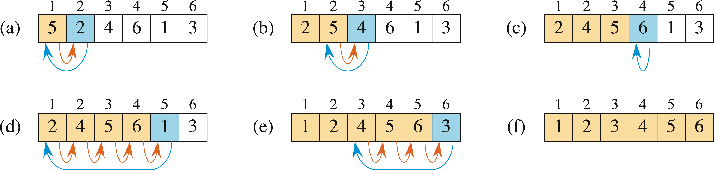
\includegraphics[angle=0]{Figures/insertion-sort.pdf}
    \caption{Visual representation of the insertion sort algorithm.}
\end{figure}

We want to prove that this is a correct algorithm. We can do this by mathematical induction using a \textit{loop invariant}.
A loop invariant is a property of a program that is true before and after each iteration of a loop. Thus, if we can formulate
the desired outcome of our algorithm (in this case, for the array to be sorted) as a loop invariant, showing that this property
is a valid loop invariant will be equivalent to proving correctness of the algorithm. To show that the loop invariant is corrent we must
show:
\newline \textbf{Initialization}: the property is true before the first iteration of the loop.
\newline \textbf{Maintenance}: if the property is true before a given iteration, it is also true before the next iteration.
\newline \textbf{Termination}: The loop terminates and gives a useful property that helps us to verify that the algorithm is correct.

For example, insertion sort is correct if the final array is sorted. Consider the following loop invariant:
\newline \textit{At the start of each iteration of the for loop, the subarray \texttt{A[1:i-1]} consists of the elements originally in \texttt{A[1:i-1]},
but in correct sorted order}.

To prove correctness of insertion sort, we prove the loop invariant always holds by induction:
\newline \textbf{Initialization}: Before the first loop iteration\footnote{In a \texttt{for} loop, this is between the counter initialization \texttt{int i = 2} and the condition
i $\leq$ n assuming a C \texttt{for} loop: \texttt{for (int i = 2; i $\leq$ n; i++)}.}, i = 2 so the left
subarray is just \texttt{A[1:i-1]} = \texttt{A[1]}, which clearly contains the original element and is sorted.
\newline \textbf{Maintenance}: Formally, we should check the while loop with a loop invariant. Informally, each interation
moves the values by one until \texttt{A[i]} is placed in the correct position. This implies that \texttt{A[1:i]}
is still sorted and contains the same elements. Thus, \textit{incrementing} i preserves this.
\newline \textbf{Termination}: To conclude our proof, we want to take the condition that terminates the loop and sub
it into the original formulation of the loop invariant above. This should give us a statement that proves the correctness of the
algorithm. The loop stops where $i > n$, or equivalently, $i = n + 1$. Subbing this in gives the following statement:
\textit{The subarray A[1:n] consists of elements originally in A[1:n] but in sorted order}. This is exactly our goal (that is, array A
has been sorted) and so this proves correctness by induction.

\textit{Linear search} solves the following \textit{searching problem}:
\newline \textbf{Input:} A sequence of $n$ numbers $\left\langle a_1, a_2, ..., a_n\right\rangle$ stored in array
A[1:n] and a value $x$.
\newline \textbf{Output:} An index $i$ such that $x$ equals A[i] or the special value \texttt{NIL} if x does not appear
in A.

Linear search scans the array from beginning to end, looking for $x$:
\begin{lstlisting}
    LINEAR-SEARCH(A, n, x)
    for i in 1 to n
        if A[i] = x
            return i
    return NIL
\end{lstlisting}

Prove its correctness with the following loop invariant: \textit{At the start of each iteration, the
subarray \texttt{A[1:i-1]} contains only elements not equal to x}. This is valid as the loop terminates when
returning either $i$ or \texttt{NIL}.


\end{document}
